\subsection{\lr{Overall Results}}
در شکل زیر می‌توانید نتیجه کلی مقایسه بین اجرای کلی و عملکرد ماشین مجازی و حقیقی را مشاهده کنید.
\begin{figure}[H]
    \centering
    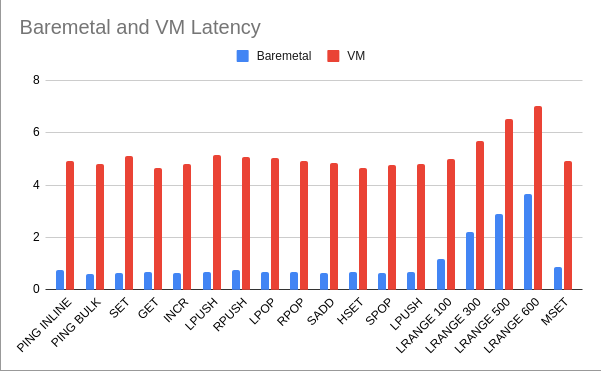
\includegraphics[scale=0.7]{pictures/redis/overall_results.png}
    \caption{مقایسه تاخیر در ماشین مجازی و حقیقی}
    \label{fig:redis:init:overall_results}
\end{figure}
همانطور که مشاهده می‌کنید تاخیر ردیس در ماشین مجازی تقریبا ۱۰ برابر ماشین حقیقی است که یعنی 
در انجام عملیات‌های دیتابیسی ماشین حقیقی عملکرد بهتری دارد که البته انتظار هم می‌رفت با توجه به اینکه ماشین حقیقی نسبت به ماشین مجازی منابع سخت‌افزاری بیشتری دارد.